\documentclass[twocolumn]{article}
\usepackage[latin1]{inputenc}
\usepackage{amsmath}
\usepackage{amsfonts}
\usepackage{amssymb}
\usepackage{array}
\usepackage{lscape}
\usepackage{tikz}
\usepackage{parskip}
\usepackage{graphicx}
\usepackage{dsfont}
\usepackage{framed}
\usepackage{upgreek}
\usepackage{listings}
\usepackage{fancyhdr}
\lstset{frame=single}
\lstset{basicstyle=\small}
\lstset{breaklines=true}
\lstset{numbers=left}
\setlength{\headheight}{15.2pt}
\setlength{\parindent}{0pt}
\usepackage{graphicx}
\usepackage{multirow}

% This section uses the cvpr styling
\usepackage{cvpr}
\cvprfinalcopy

% Uncomment this for NIPS
%\usepackage{nips12submit_e}
%\nipsfinalcopy

% This is for debugging purposes to throw color in here so we don't forget certain things.
\usepackage{color}

\setcounter{secnumdepth}{2}
\newcommand{\tab}{\hspace*{2em}}

\newcommand{\sectionfile}[3]{\section{#1} \label{sec:#2} \input{#3}}

\newcommand{\subsectionfile}[3]{\subsection{#1} \label{sec:#2} \input{#3}}

\title{TourDruid}
\author{\textbf{Peter Sugihara}\\ \textsc{pys2105}
\and \textbf{Cody De La Vara}\\ \textsc{cgd2120}
\and \textbf{Joe Ellis}\\ \textsc{jge2105}
\and \textbf{Matthew Piziak}\\ \textsc{mjp2175}}

% Comment this out if not using NIPS
%\nipsfinalcopy

\begin{document}

\maketitle

\begin{abstract}

With the ubiquitous use of handheld communication devices equipped with built in cameras we are entering into a world where sharing of visual content is becoming an hourly activity.
The platforms for sharing visual content such as Twitter, Facebook, and Instagram have been in development for multiple years and are now incredibly quick and reliable.
However, although a multitude of pictures are now available to us much less work has gone into actually analyzing this visual content and creating a useful system that is fast and intuitive based off of Computer Vision principles.
To address this issue we present TourDruid, an application built for iPhone that allows a Columbia University tourist to take a picture of a building on the CU campus, and the TourDruid will return the name of the building, pertinent information about this building, and the location of the building on Columbia Campus.
Using our proposed algorithm on a novel dataset we are able to achieve a 10-fold cross validation accuracy of {\color{red} XXX }.  
After a picture is chosen by a user our system returns the results in {\color{red} XXX}, which is fast enough in our opinion to make this application useful to a general tourist.
This application has been sent to the Apple App Store for verification and once available can be found by searching TourDruid.

\end{abstract}

%\lstlistoflistings
% we can add source code listings if we desire

\newpage

% This is how you add a new section.
\sectionfile{Introduction}{introduction}{introduction.tex}

\begin{figure}
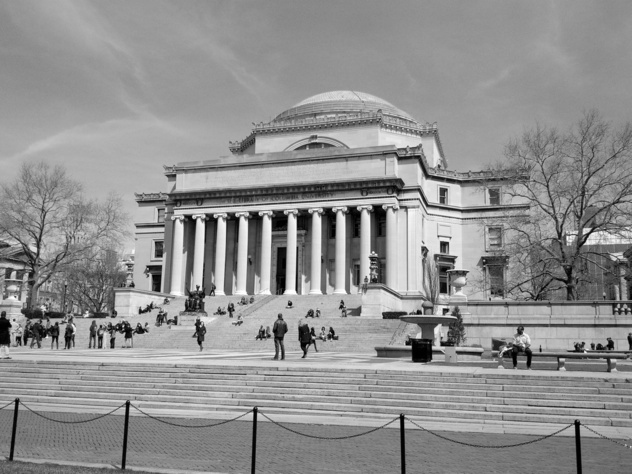
\includegraphics[width=40mm]{sample_data1.jpg}
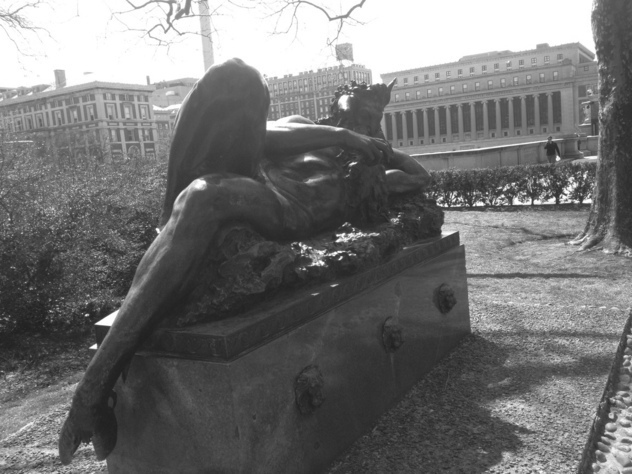
\includegraphics[width=40mm]{sample_data2.jpg}
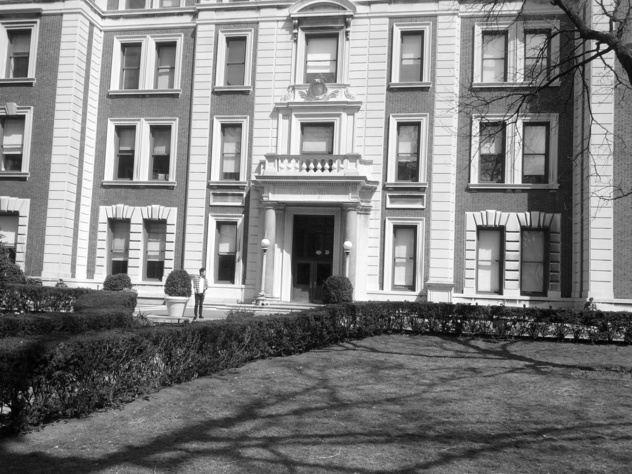
\includegraphics[width=40mm]{sample_data3.jpg}
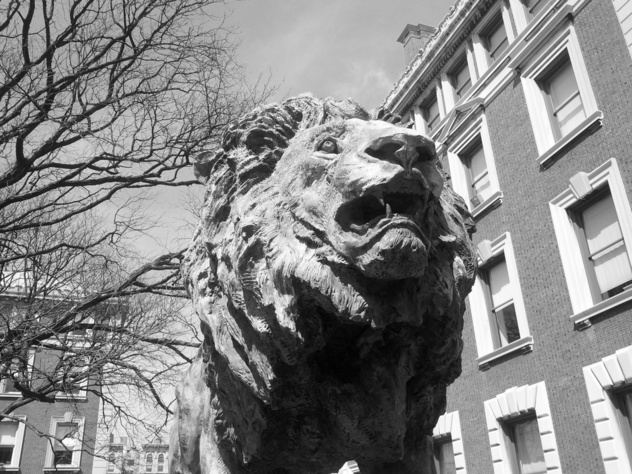
\includegraphics[width=40mm]{sample_data4.jpg}
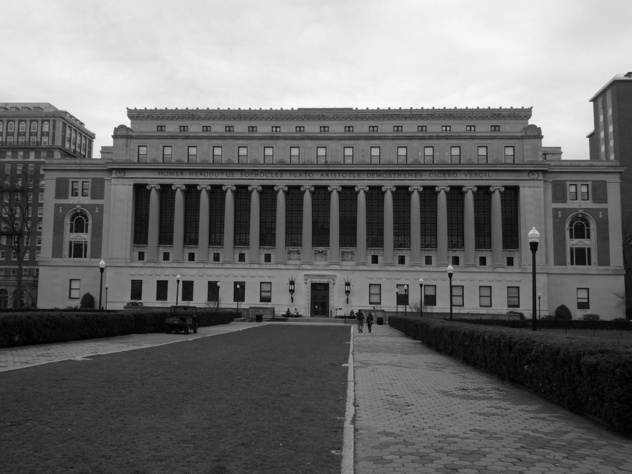
\includegraphics[width=40mm]{sample_data5.jpg}
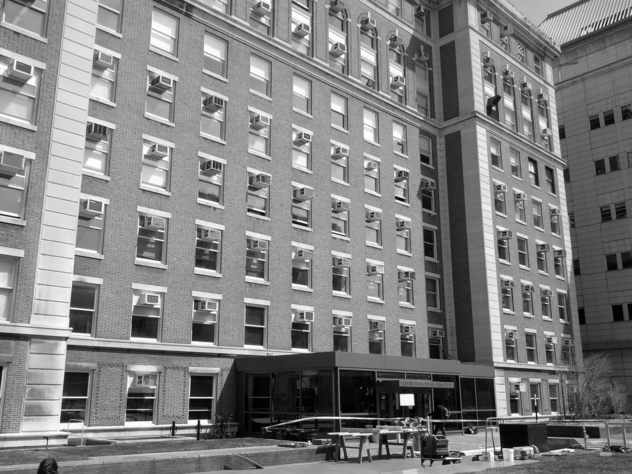
\includegraphics[width=40mm]{sample_data6.jpg}
\caption{Sample images from our dataset post-processing}
\label{overflow}
\end{figure}
\sectionfile{Dataset}{dataset}{dataset.tex}
\sectionfile{Procedure}{procedure}{procedure.tex}
\begin{figure}
%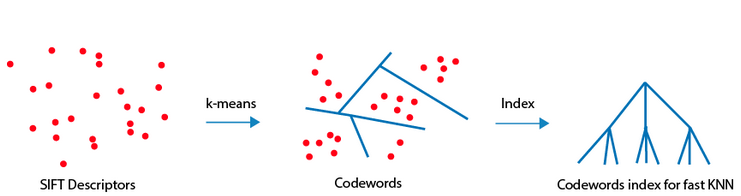
\includegraphics[width=90mm]{procedure1.png}
%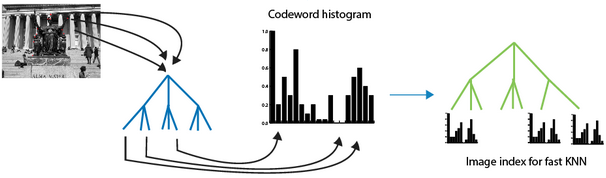
\includegraphics[width=90mm]{procedure2.png}
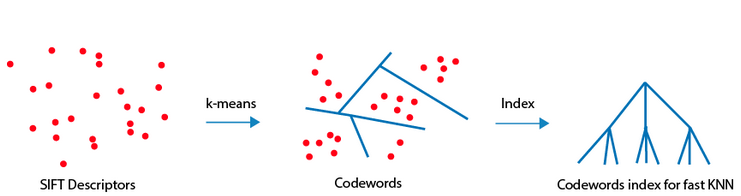
\includegraphics[width=90mm]{procedure1.png}
\caption{Procedure pipeline 1}
\end{figure}
\begin{figure}
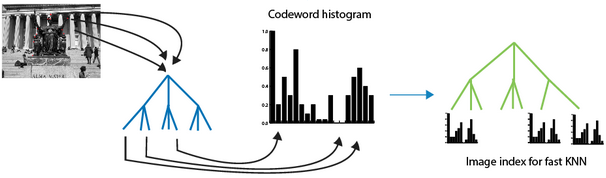
\includegraphics[width=90mm]{procedure2.png}
\caption{Procedure pipeline 2}
\label{overflow}

\end{figure}
\sectionfile{Results}{results}{results.tex}

\begin{figure}
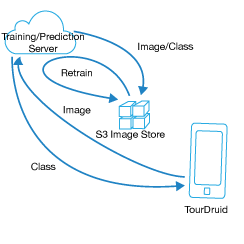
\includegraphics[width=86mm]{app_arch.png}

\caption{Application Architecture Diagram}
\label{overflow}

\end{figure}
\sectionfile{Application Architecture}{application_architecture}{application_architecture.tex}
\sectionfile{Future Work}{future_work}{future.tex}
\sectionfile{Conclusion}{conclusion}{conclusion.tex}

\nocite{*}
{\small
\bibliographystyle{ieee}
\bibliography{TourDruidbib}
}


\end{document}